%  LaTeX support: latex@mdpi.com 
%  For support, please attach all files needed for compiling as well as the log file, and specify your operating system, LaTeX version, and LaTeX editor.

%=================================================================
\documentclass[sensors,article,submit,moreauthors,pdftex]{Definitions/mdpi} 

% For posting an early version of this manuscript as a preprint, you may use "preprints" as the journal and change "submit" to "accept". The document class line would be, e.g., \documentclass[preprints,article,accept,moreauthors,pdftex]{mdpi}. This is especially recommended for submission to arXiv, where line numbers should be removed before posting. For preprints.org, the editorial staff will make this change immediately prior to posting.

%--------------------
% Class Options:
%--------------------
%----------
% journal
%----------
% Choose between the following MDPI journals:
% acoustics, actuators, addictions, admsci, adolescents, aerospace, agriculture, agriengineering, agronomy, ai, algorithms, allergies, analytica, animals, antibiotics, antibodies, antioxidants, appliedchem, applmech, applmicrobiol, applnano, applsci, arts, asi, atmosphere, atoms, audiolres, automation, axioms, batteries, bdcc, behavsci, beverages, biochem, bioengineering, biologics, biology, biomechanics, biomedicines, biomedinformatics, biomimetics, biomolecules, biophysica, biosensors, biotech, birds, bloods, brainsci, buildings, businesses, cancers, carbon, cardiogenetics, catalysts, cells, ceramics, challenges, chemengineering, chemistry, chemosensors, chemproc, children, civileng, cleantechnol, climate, clinpract, clockssleep, cmd, coatings, colloids, compounds, computation, computers, condensedmatter, conservation, constrmater, cosmetics, crops, cryptography, crystals, curroncol, cyber, dairy, data, dentistry, dermato, dermatopathology, designs, diabetology, diagnostics, digital, disabilities, diseases, diversity, dna, drones, dynamics, earth, ebj, ecologies, econometrics, economies, education, ejihpe, electricity, electrochem, electronicmat, electronics, encyclopedia, endocrines, energies, eng, engproc, entropy, environments, environsciproc, epidemiologia, epigenomes, fermentation, fibers, fire, fishes, fluids, foods, forecasting, forensicsci, forests, fractalfract, fuels, futureinternet, futuretransp, futurepharmacol, futurephys, galaxies, games, gases, gastroent, gastrointestdisord, gels, genealogy, genes, geographies, geohazards, geomatics, geosciences, geotechnics, geriatrics, hazardousmatters, healthcare, hearts, hemato, heritage, highthroughput, histories, horticulturae, humanities, hydrogen, hydrology, hygiene, idr, ijerph, ijfs, ijgi, ijms, ijns, ijtm, ijtpp, immuno, informatics, information, infrastructures, inorganics, insects, instruments, inventions, iot, j, jcdd, jcm, jcp, jcs, jdb, jfb, jfmk, jimaging, jintelligence, jlpea, jmmp, jmp, jmse, jne, jnt, jof, joitmc, jor, journalmedia, jox, jpm, jrfm, jsan, jtaer, jzbg, kidney, land, languages, laws, life, liquids, literature, livers, logistics, lubricants, machines, macromol, magnetism, magnetochemistry, make, marinedrugs, materials, materproc, mathematics, mca, measurements, medicina, medicines, medsci, membranes, metabolites, metals, metrology, micro, microarrays, microbiolres, micromachines, microorganisms, minerals, mining, modelling, molbank, molecules, mps, mti, nanoenergyadv, nanomanufacturing, nanomaterials, ncrna, network, neuroglia, neurolint, neurosci, nitrogen, notspecified, nri, nursrep, nutrients, obesities, oceans, ohbm, onco, oncopathology, optics, oral, organics, osteology, oxygen, parasites, parasitologia, particles, pathogens, pathophysiology, pediatrrep, pharmaceuticals, pharmaceutics, pharmacy, philosophies, photochem, photonics, physchem, physics, physiolsci, plants, plasma, pollutants, polymers, polysaccharides, proceedings, processes, prosthesis, proteomes, psych, psychiatryint, publications, quantumrep, quaternary, qubs, radiation, reactions, recycling, regeneration, religions, remotesensing, reports, reprodmed, resources, risks, robotics, safety, sci, scipharm, sensors, separations, sexes, signals, sinusitis, smartcities, sna, societies, socsci, soilsystems, solids, sports, standards, stats, stresses, surfaces, surgeries, suschem, sustainability, symmetry, systems, taxonomy, technologies, telecom, textiles, thermo, tourismhosp, toxics, toxins, transplantology, traumas, tropicalmed, universe, urbansci, uro, vaccines, vehicles, vetsci, vibration, viruses, vision, water, wevj, women, world 

%---------
% article
%---------
% The default type of manuscript is "article", but can be replaced by: 
% abstract, addendum, article, book, bookreview, briefreport, casereport, comment, commentary, communication, conferenceproceedings, correction, conferencereport, entry, expressionofconcern, extendedabstract, datadescriptor, editorial, essay, erratum, hypothesis, interestingimage, obituary, opinion, projectreport, reply, retraction, review, perspective, protocol, shortnote, studyprotocol, systematicreview, supfile, technicalnote, viewpoint, guidelines, registeredreport, tutorial
% supfile = supplementary materials

%----------
% submit
%----------
% The class option "submit" will be changed to "accept" by the Editorial Office when the paper is accepted. This will only make changes to the frontpage (e.g., the logo of the journal will get visible), the headings, and the copyright information. Also, line numbering will be removed. Journal info and pagination for accepted papers will also be assigned by the Editorial Office.

%------------------
% moreauthors
%------------------
% If there is only one author the class option oneauthor should be used. Otherwise use the class option moreauthors.

%---------
% pdftex
%---------
% The option pdftex is for use with pdfLaTeX. If eps figures are used, remove the option pdftex and use LaTeX and dvi2pdf.

%%%% ДЛЯ РУССКОГО ТЕКСТА закомментировать потом!
%\usepackage{inputenc}
%\usepackage[T2A,T1]{fontenc}
%\usepackage[english,russian]{babel}
%\usepackage{cmap}
%%%%

%=================================================================
% MDPI internal commands
\firstpage{1} 
\makeatletter 
\setcounter{page}{\@firstpage} 
\makeatother
\pubvolume{1}
\issuenum{1}
\articlenumber{0}
\pubyear{2021}
\copyrightyear{2020}
%\externaleditor{Academic Editor: Firstname Lastname} % For journal Automation, please change Academic Editor to "Communicated by"
\datereceived{} 
\dateaccepted{} 
\datepublished{} 
\hreflink{https://doi.org/} % If needed use \linebreak
%------------------------------------------------------------------
% The following line should be uncommented if the LaTeX file is uploaded to arXiv.org
%\pdfoutput=1

%=================================================================
% Add packages and commands here. The following packages are loaded in our class file: fontenc, inputenc, calc, indentfirst, fancyhdr, graphicx, epstopdf, lastpage, ifthen, lineno, float, amsmath, setspace, enumitem, mathpazo, booktabs, titlesec, etoolbox, tabto, xcolor, soul, multirow, microtype, tikz, totcount, changepage, paracol, attrib, upgreek, cleveref, amsthm, hyphenat, natbib, hyperref, footmisc, url, geometry, newfloat, caption

%=================================================================
%% Please use the following mathematics environments: Theorem, Lemma, Corollary, Proposition, Characterization, Property, Problem, Example, ExamplesandDefinitions, Hypothesis, Remark, Definition, Notation, Assumption
%% For proofs, please use the proof environment (the amsthm package is loaded by the MDPI class).

%=================================================================
% Full title of the paper (Capitalized)
\Title{Optimization of Turbulence Model Parameters Using the Global Search Method Combined with Machine Learning}

% MDPI internal command: Title for citation in the left column
\TitleCitation{Optimization of Turbulence Model Parameters Using the Global Search Method Combined with Machine Learning}

% Author Orchid ID: enter ID or remove command
\newcommand{\orcidauthorA}{0000-0001-5273-2471} % Add \orcidA{} behind the author's name
\newcommand{\orcidauthorB}{0000-0002-8736-0652} % Add \orcidB{} behind the author's name
\newcommand{\orcidauthorC}{0000-0002-0722-6884} % Add \orcidC{} behind the author's name

\newcommand{\orcidauthorD}{0000-0002-5771-4114} % Add \orcidD{} behind the author's name
\newcommand{\orcidauthorE}{0000-0001-5525-5180} % Add \orcidF{} behind the author's name
\newcommand{\orcidauthorF}{0000-0001-9568-7121} % Add \orcidG{} behind the author's name

% Authors, for the paper (add full first names)
\Author{Konstantin Barkalov $^{1}$\orcidA{}, Ilya Lebedev $^{1}$\orcidB{}, Marina Usova$^{1}$\orcidC{}, Daria Romanova$^2$\orcidD{}, Daniil~Ryazanov$^2$\orcidF{} and Sergei~Strijhak$^2$\orcidE{}}

% MDPI internal command: Authors, for metadata in PDF
\AuthorNames{Konstantin Barkalov, Ilya Lebedev, Marina Usova, Daria Romanova, Daniil~Ryazanov and Sergei~Strijhak}

% MDPI internal command: Authors, for citation in the left column
\AuthorCitation{Barkalov, K.; Lebedev, I., Usova, M.; Romanova D.; Ryazanov D.; Strijhak S.}
% If this is a Chicago style journal: Lastname, Firstname, Firstname Lastname, and Firstname Lastname.

% Affiliations / Addresses (Add [1] after \address if there is only one affiliation.)
\address{%
$^{1}$ \quad Department of Mathematical Software and Supercomputing Technologies, Lobachevsky University, 603950 Nizhni Novgorod, Russia; konstantin.barkalov@itmm.unn.ru (K.B.), ilya.lebedev@itmm.unn.ru (I.L.), marina.usova@itmm.unn.ru (M.U.)\\
$^{2}$ \quad Institute For System Programming of Russian Academy of Science, 109004, Moscow, Russia; Ryazanov Daniil ryazanov@ispras.ru (R.D.), Sergei Strijhak s.strijhak@ispras.ru (S.S.), Romanova Daria romanova.d@ispras.ru (Rom.D.)}

% Contact information of the corresponding author
\corres{Correspondence: Ryazanov Daniil, ryazanov@ispras.ru;}

% Current address and/or shared authorship
%\firstnote{Current address: Affiliation 3} 
%\secondnote{These authors contributed equally to this work.}
% The commands \thirdnote{} till \eighthnote{} are available for further notes

%\simplesumm{} % Simple summary

%\conference{} % An extended version of a conference paper

% Abstract (Do not insert blank lines, i.e. \\) 

\abstract{The paper considers the slope flow simulation and the problem of finding the optimal parameters values of this mathematical model. The slope flow is modeled using the finite volume method the averaged Reynolds equations model and the $k-\omega\ SST$ turbulence model. The Root Mean Square Error of the calculated flow velocity profile is considered as the objective function in the optimization problem. The analytical form of this function is not known and the calculation of its values involves time-consuming numerical simulation. The optimal values of the coefficients of the turbulence model were found using the global search algorithm. To speed up the optimization procedure, the objective function was approximated using artificial neural network. The optimal coefficients of the turbulence model for slope flows were obtained with virtual sensors, and the calculated data were compared with the experimental ones. An interdisciplinary approach was utilized, which helped to find the optimal values of six turbulence model parameters using OpenFOAM and Globalizer software.}


% Keywords
\keyword{global optimization; artificial neural network; function approximation; finite volume method; CFD} 

% The fields PACS, MSC, and JEL may be left empty or commented out if not applicable
%\PACS{J0101}
%\MSC{}
%\JEL{}

%%%%%%%%%%%%%%%%%%%%%%%%%%%%%%%%%%%%%%%%%%
% Only for the journal Diversity
%\LSID{\url{http://}}

%%%%%%%%%%%%%%%%%%%%%%%%%%%%%%%%%%%%%%%%%%
% Only for the journal Applied Sciences:
%\featuredapplication{Authors are encouraged to provide a concise description of the specific application or a potential application of the work. This section is not mandatory.}
%%%%%%%%%%%%%%%%%%%%%%%%%%%%%%%%%%%%%%%%%%

%%%%%%%%%%%%%%%%%%%%%%%%%%%%%%%%%%%%%%%%%%
% Only for the journal Data:
%\dataset{DOI number or link to the deposited data set in cases where the data set is published or set to be published separately. If the data set is submitted and will be published as a supplement to this paper in the journal Data, this field will be filled by the editors of the journal. In this case, please make sure to submit the data set as a supplement when entering your manuscript into our manuscript editorial system.}

%\datasetlicense{license under which the data set is made available (CC0, CC-BY, CC-BY-SA, CC-BY-NC, etc.)}

%%%%%%%%%%%%%%%%%%%%%%%%%%%%%%%%%%%%%%%%%%
% Only for the journal Toxins
%\keycontribution{The breakthroughs or highlights of the manuscript. Authors can write one or two sentences to describe the most important part of the paper.}

%%%%%%%%%%%%%%%%%%%%%%%%%%%%%%%%%%%%%%%%%%
% Only for the journal Encyclopedia
%\encyclopediadef{Instead of the abstract}
%\entrylink{The Link to this entry published on the encyclopedia platform.}
%%%%%%%%%%%%%%%%%%%%%%%%%%%%%%%%%%%%%%%%%%

\begin{document}
%%%%%%%%%%%%%%%%%%%%%%%%%%%%%%%%%%%%%%%%%%
\section{Introduction}

The climate change is accompanied by dangerous natural phenomena, which occur more and more often. These phenomena affect human life and daily activities inevitably. The investigations of these issues include construction of mathematical models and analysis of geophysical data as well as of data from numerical and field experiments. Current trend in the analysis of geodata is associated with the use of machine learning algorithms and artificial neural networks.

The landslides, mudflows, and avalanches are classified as dangerous geological phenomena. These are the slope processes associated with the separation of rocks, movement of the ones along the slope under the influence of gravity and leading to irreversible changes in the relief. The study of the descent of landslides, mudflows, and avalanches as well as prediction and detection of the ones are urgent due to the impact of these dangerous phenomena on human life and urban infrastructure. The landslides are distinguished by the main causes of the ones. These are: abrasive, erosional, man-made, and natural-man-made.According to the mechanism of displacement, block landslides, shears, stretching, and liquefaction are distinguished, respectively \cite{Pendin2015}.

The data show that in total $55\,997$ people were killed in $4\,862$ distinct landslide events covering the period from January 2004 to December 2016. The spatial distribution of landslides is heterogeneous, with Asia representing the dominant geographical area \cite{Froude2018}.

A large number of landslides, avalanches, and mudflows occur in European countries (Switzerland, Austria, Italy, France, and Iceland). Similar dangerous phenomena occur in Russia, for example, in Krasnodar Territory of the Russian Federation and in  North Caucasus due to heavy rainfalls in these regions where mountainous terrain are present and in connection with the development of the territory (linear and areal objects) in recent years \cite{hungr2005landslide}.  The amount of precipitation was outstanding in the above territories of Russia (Sochi, Krasnaya Polyana) in 2021. This led to the flooding of mountain rivers and increased the risk of slope flows. Catastrophic descents of mudflows occured that led to damage of the road equipment and to overlap of the roadways \cite{Harch2020}.

The mudflows are one of the most complex exogenous geological processes, which integrate the actions of other geological processes. The mudflow is a complex heterogeneous structure consisting of liquid and solid components. The solid fraction consists of mineral particles, which are nonuniform from the granulometric viewpoint.

The most well-known landslide problem involves assessing the stability of a landslide slope for static conditions and seismic impact. Modeling the descent of the slope flow allows predicting the destruction caused by this phenomenon, correctly locating protective structures and vital objects.

The most well-known landslide problem involves assessing the stability of a landslide slope for static conditions and seismic impact. Modeling the descent of the slope flow allows predicting the destruction caused by this phenomenon and locating the protective structures and vital objects correctly. Such problems are solved using finite-differences methods \cite{Bernander2016}, finite volume method \cite{liu2007application}, descrete elements \cite{Liu2020} of cellular automata \cite{piegari2006cellular}, and hybrid methods. The mudflows can be modeled using a two-fluid model based on the Volume of Fluid model \cite{Hirt1981}. The methods listed above are implemented in various commercial and open source software packages MN2D \cite{Naaim2002}, TITAN2D \cite{Pitman2003}, and RAMMS.

Previously, the study of avalanches was carried out using computational fluid dynamics methods for Newtonian fluids and analysis of observation data including the historical data on avalanches in Japan \cite{Oda2011, Yamaguchi2017}. Similar work was carried out on avalanches in Switzerland, Austria, and Italy. A series of works on the study of avalanches using a laboratory experiment in special trays and measuring equipment for studying avalanches in Iceland were carried out University of Iceland  \cite{IceThesKatr, IceThesJon}. An experiment with the descent of a snow-water stream in Davos, Switzerland was described in \cite{Jaedicke2006}. Measurements were made for the flow depth for a dry snow avalanche and for a snow-water flow.

Cheung et al. \cite{Cheung2011} used Bayesian analysis for the calibration of the Spalart–Allmaras turbulence model coefficients, and model inadequacy, to reproduce the turbulent boundary layer profile over the flat plate. Among similar works, the coefficients were already calibrated in the $k-\varepsilon$ turbulence model when studying the process of the propagation of impurities in urban development \cite{Guillas2014}.

Bayesian analysis has been proposed to address the question of RANS turbulence models (The $k–\varepsilon$ model with Launder–Sharma damping functions, The Wilcox $k–\omega$ model, the Spalart–Allmaras and Baldwin–Lomax models) calibration towards increased prediction accuracy without computational efficiency loss \cite{Edeling2014a,Edeling2014b}  de Zordo–Banliat et al. \cite{deZordoBanliat2020}  applied Bayesian analysis to compressor cascades to produce a set of calibrated turbulence model parameters with emphasis on the turbulence model inadequacy.

Kotaro Matsui et al. \cite{Matsui2021} proposed a new set of calibrated coefficients that improved the ability of Spalart-Allmaras model to predict a corner flow separation of a compressor cascade. A comprehensive review of turbulence model uncertainties is given in paper of Xiao and Cinnella \cite{Xiao2019}. 


A comprehensive analysis of climatic, geological, and hydrological data was applied to model and predict the slope flows. In the scope of recent trends, huge streams of data received from satellites from the experiments, and from mathematical modeling are processed using machine learning, which makes it possible to develop efficient models of these processes \cite{GeoML, Ma2020}.

Methods based on convolutional neural networks (CNN) are able to extract stable spatial and spectral features \cite{Maggiori2017}. The combination of satellite image and topographic data can be used to generalize the extracted features in order to identify the slope flows in the satellite images \cite{Qin2021, Prakash2021}.

The slope flow model, as a rule, includes several parameters, the values of which cannot be specified in advance but can be selected based on the correspondence of the numerical calculation results to the experimental data available. Such a problem is a global optimization one with a black box objective function because the specific type of the objective function is not known, there is an algorithm for calculating its values only.

The complexity of the phenomena and processes under study is reflected in the complexity of the corresponding mathematical models and numerical methods for the analysis of these ones. Currently, the main (and often the only possible) tool for such an analysis is supercomputer modeling of the object behavior. Open source software is used widely in this purpose. OpenFOAM (an open platform for numerical modeling of continuum mechanics problems) is a well-known example of open source software of this kind \cite{Weller1998}. 

%ННГУ
% Если будет предыдущая связка, то вот этот абзац можно и опустить, и начать - со следующего,
Growth of performance of modern supercomputer systems goes in parallel with complication of complication of mathematical models of the processes considered that makes performing even a single model calculation (a \textit{trial}) a computation-costly operation. Consequently, the choice of the optimal values of the model parameters in reasonable time cannot be completed by trying all possible variants by grid method, i.e. by search on some regular grid in a range of variation of the parameters. Impossibility of performing a large number of search trials requires applying efficient search algorithms, which would provide an acceptable estimate of a problem solution at relatively small number of trials using available computational resources.

%ННГУ - начать можно отсюда
It is worth noting that majority of existing methods for search of the optimum of time-consuming black-box functions have some drawbacks. Gradient-based algorithms cannot be used in many cases just because the derivatives of an objective function are unknown while the finite-difference approximations of these ones are too computation costly. At the same time, in general, the gradient-based methods provide the finding of a local optimal problem solution only.
Classical direct search methods, which don't require the derivatives, e.g. Nelder-Mead method \cite{NelderMead} or Hooke-Jeeves method \cite{HookJeeves}, are the local ones as well. As a rule, the application of these methods for solving the global optimization problems involves several restarts from nodes of a random grid that requires a large number of trials. 

Deterministic methods of Lipschitz global optimization, such as DIRECT \cite{Jones2009}, non-uniform coverages method \cite{Evtushenko2009, Evtushenko2013}, diagonal \cite{Sergeyev2017}, and simplicial \cite{Zilinskas2014} methods guarantee (in the limit) convergence to the global solution of the problem but may require a large number of the search trials.
Finally, heuristic methods, e.g. differential evolution or simulated annealing, also require very large number of computations of the functions to obtain good estimates of the solutions in the global optimization problems and loose in quality to the deterministic algorithms at the same time \cite{Sergeyev2018,Kvasov2018}.

So far, direct application of the optimization algorithms to the search of the minima of the time-consuming function may appear too computation-costly when the performing of a single trial takes much computation time.
A construction of an approximation of the objective function (also known as a response surface model or a metamodel or a surrogate model), computing the values of which is an inexpensive operation is a well known method to overcome this problem. The approximation is used further to find the minimum.
There are many variants of constructing the approximations for multivariate functions. These are various interpolation methods utilizing polynomials, splines, radial basis functions, Kriging, as well as various regression models. Many of these algorithms are used in developing the global optimization methods.

For example, the use of the radial basis functions has been considered in details in \cite{Gutmann2001,Regis2005}. In \cite{Jones1998,UrRehman2014,Ollar2017_1}, Kriging-based methods have been proposed. A novel approach to constructing the metamodels and trust-region methods based on these ones has been presented in \cite{Polynkin2012,Ollar2017_2,Toropov2018}. 

In the present study, we used efficient global search algorithm (GSA) \cite{Strongin2000,Sergeyev2013} for solving the Lipschitz global optimization problems combined with a function approximations based on the regression models. At the first search stage, GSA worked with the objective function as a direct method. Then, an approximation of the objective function was constructed on the base on the accumulated information. This approximation was used at the second stage of the search.
To construct the approximations, we applied Neural Network Regression (NNR).

To study the parameters of slope flows, it is advisable to use interdisciplinary approaches from the fields of computational and experimental hydrodynamics, optimization theory, parallel computing and neural networks. This paper uses the results of an experiment in a chute with a different angle of inclination, a mathematical model for modeling a two-phase flow, global optimization methods and an artificial neural network. The mathematical model is based on the averaged Reynolds equations and a two-parameter turbulence model. 

Existing turbulence models contain a number of constants that were calibrated for canonical flows such as air flow around various profiles, flows in pipes and channels, etc. \cite{LaunderSpalding1974, Tahry1983, LaunderMorseRodiSpaldiug1972}. Calibration of turbulence models coefficients for calculating flows of a Newtonian media with a free surface on mountain slopes has not been performed. In this work, the coefficients of the $k-\omega\ SST$ turbulence model were optimized for calculating the turbulent fluid flow in the chute.

The main part of the paper has the following structure. 
Section 2 contains a description of the experiment. Section 3 describes mathematical model of turbulent two-phase flows. In Section 4 contains the details of numerical methods. 
Section 5 describes the results of numerical experiments. 
Section 6 concludes the paper.


%%%%%%%%%%%%%%%%%%%%%%%%%%%%%%%%%%%%%%%%%%
\section{The Experiment in Inclined Chute}

Experimental installations are used to study the parameters of slope flows. The objects of study are such measurements as flow depth, flow velocity, force of interaction with an obstacle. Such measurements as flow depth, flow velocity, impact force on an obstacle become the object of study. In our study, the velocity profile is studied.

An experiment setup at the Research Institute of Mechanics, Lomonosov Moscow State University was used for this purpose. In the experiment, a turbulent fluid flow descended along a chute with a constant slope. The experiment was carried out for several different slope angles. The chute has the following geometry: the length 1~m, the width 12~cm, and the side heights 10~cm. The chute area to analyze is between two points of velocity and depth measurements located at the distances of 23~cm and 82~cm from the top edge. The schematic representation of the experiment is shown in Figure~\ref{NIIMexLinearUProfileInlet}. Tap water was used for the experiment.

\begin{figure}[H]	
\widefigure
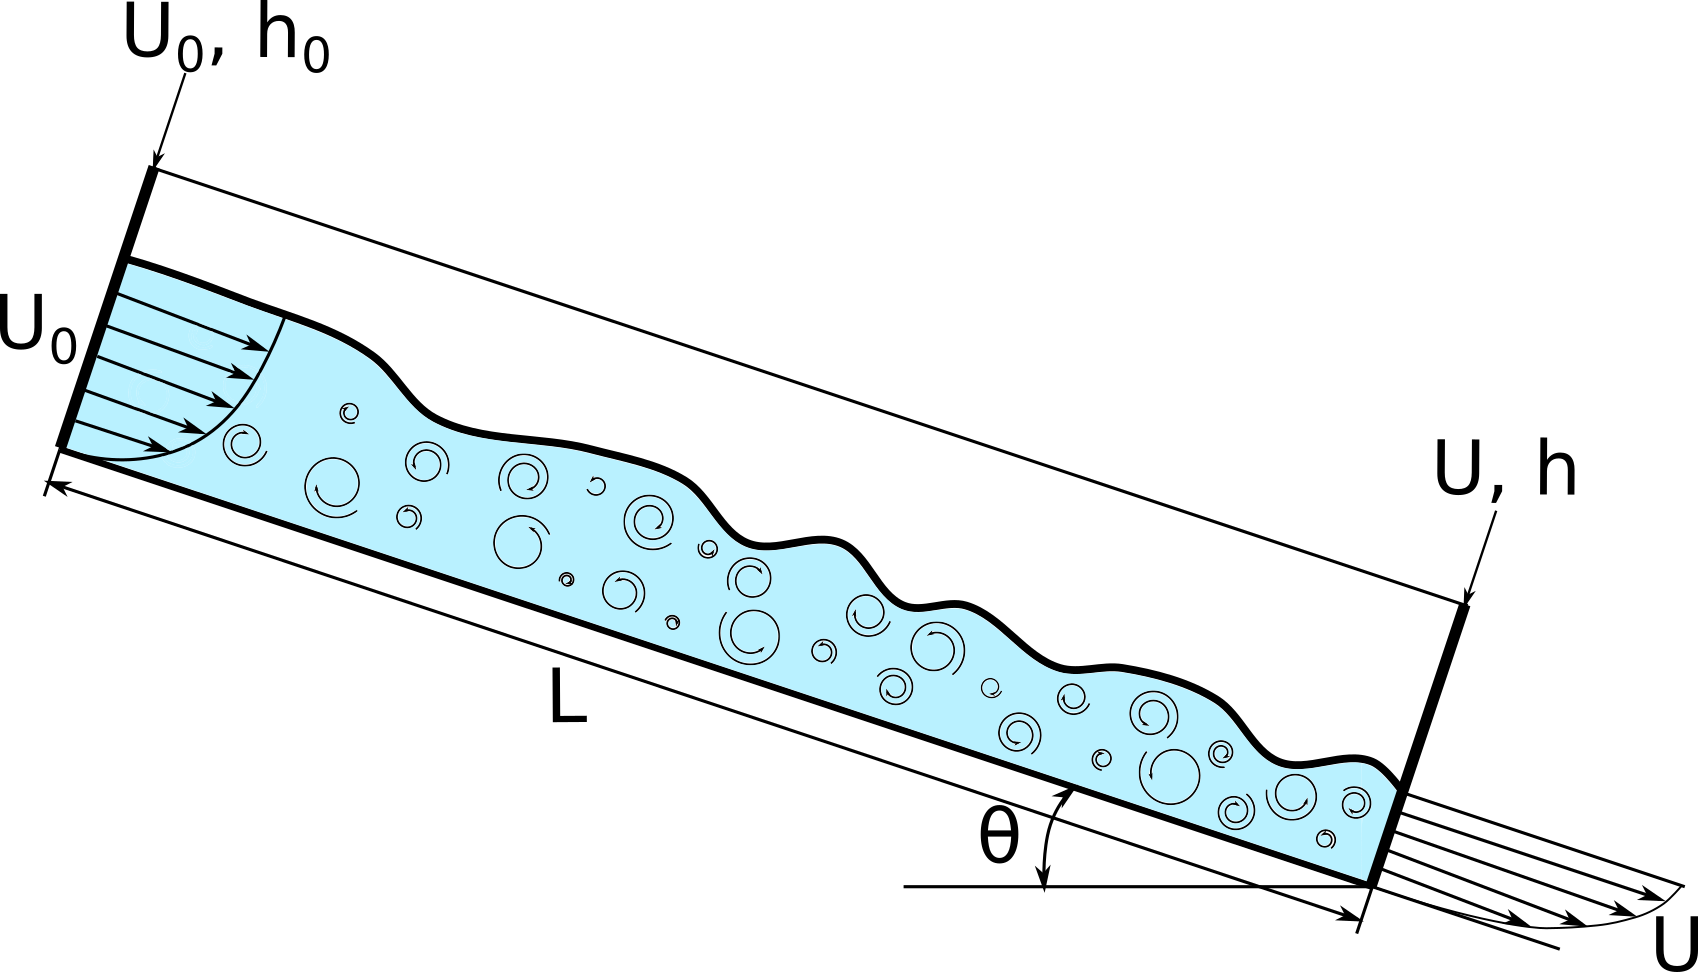
\includegraphics[width=10 cm]{NIIMexLinearUProfileInlet.png}
\caption{Experiment chute scheme\label{NIIMexLinearUProfileInlet}}
\end{figure}

%Было проведено 3 серии экспериментов, в которых менялся угол наклона склона, начальная глубина потока, начальный профиль потока, как показано в таблице \ref{tabNIIMexLinear}
Three series of experiments were done; the initial flow profile, the initial flow depth, the slope angle were varied as shown in Table~\ref{tabNIIMexLinear}.

%\begin{table}[H]
%	\caption{Параметры расчётов}
%	\label{tabNIIMexLinear}
%	\begin{center}
%		\begin{tabular}{ | c | c | c | } 
%			\hline
%			$u_0$ среднее по глубине, м/с & $h_0$, мм & $\theta$\\
%			\hline
%			1.63 & 4.20 & 25$^\circ$\\
%			2.00 & 4.95 & 28$^\circ$\\
%			1.78 & 3.45 & 33$^\circ$\\
%			\hline
%		\end{tabular}
%	\end{center}
%\end{table}

\begin{specialtable}[H]
    \centering
	\caption{Parameters of the experiments\label{tabNIIMexLinear}}
	\begin{tabular}{  c  c  c  }
	\toprule
	\textbf{$\boldsymbol{u_0}$, m/s}	& \textbf{$\boldsymbol{h_0}$, mm}	& \textbf{$\boldsymbol{\theta}$}\\
	\midrule
	1.63 & 4.20 & 25$^\circ$\\
	2.00 & 4.95 & 28$^\circ$\\
	1.78 & 3.45 & 33$^\circ$\\
	\bottomrule
	\end{tabular}
\end{specialtable}

Where $u_0$ is a depth-averaged velocity. $h_0$~--- the flow depth. $\theta$~--- the slope inclination angle.

%%%%%%%%%%%%%%%%%%%%%

%ННГУ

\section{Mathematical model}\label{math_model}

%Для расчёта эксперимента поставленного в НИИ Механики МГУ используются осреднённые по Рейнольдсу уравнения Навье-Стокса. Для получения значений тензора напряжений Рейнольдса используется замыкание в виде $k-\omega\ SST$ модели турбулентности. Положение свободной поверхности потока определяется с использованием метода объёма жидкости VOF (Volume Of Fluid), предложенного Хиртом и Николсом в 1981 году \cite{HirtNichols1981}. В данном методе используется величина объёмной доли фазы воды $\alpha$ в ячейке для определения свободной поверхности таким образом, что при $\alpha>0.6$ считается что ячейка заполнена жидкостью, в противном случае~--- воздухом.
The Reynolds-averaged Navier-Stokes equations were used to model the experiment carried out at the Research Institute of Mechanics of Lomonosov Moscow State University. The $k-\omega\ SST$ turbulence model was used to obtain the values of the Reynolds stress tensor. The position of the free surface of the flow is determined using the VOF (Volume Of Fluid) method proposed by Hirt and Nichols in 1981 \cite{HirtNichols1981}. In this method, the volume fraction of water phase $\alpha$ in the cell is used to determine the free surface so that if $\alpha>0.6$, the cell is considered to be filled with liquid, otherwise --- to be filled with air.


To describe the flow, the system of equations \eqref{vofKWSST} is used, which consists of the continuity equation for a mixture, the volume phase fraction transfer equation, the momentum conservation equation, the turbulent kinetic energy and specific dissipation rate equations.

\begin{equation}
	\label{vofKWSST}
	\left\{
		\begin{aligned}
			&\boldsymbol{\nabla} \cdot \bar{\boldsymbol{u}} = 0,\\
			&\frac{\partial \alpha}{\partial t} + \boldsymbol{\nabla} \cdot (\bar{\boldsymbol{u}} \alpha) = 0,\\
			&\frac{\partial (\rho \bar{\boldsymbol{u}})}{\partial t} + \boldsymbol{\nabla} \cdot (\rho \bar{\boldsymbol{u}} \bar{\boldsymbol{u}}) = -\boldsymbol{\nabla} \bar{p} + \boldsymbol{\nabla} \cdot \bar{\boldsymbol{\tau}} + \rho \bar{\boldsymbol{f}},\\
			&\frac{\partial (\rho k)}{\partial t} + \boldsymbol{\nabla} \cdot (\rho \bar{\boldsymbol{u}} k) = \widetilde{P}_k - \beta^*\rho k \omega + \boldsymbol{\nabla} \cdot \left( (\mu + \alpha_k \mu_t) \boldsymbol{\nabla} k \right),\\
			&\frac{\partial (\rho \omega)}{\partial t}  + \boldsymbol{\nabla} \cdot ( \rho \bar{\boldsymbol{u}} \omega) = \gamma \rho \dot{s}^2 - \beta \rho \omega^2 + \boldsymbol{\nabla} \cdot \left( (\mu + \alpha_\omega \mu_t) \boldsymbol{\nabla} \omega \right) + \\
			&+2 (1 - F_1) \rho \alpha_{\omega 2} \frac{1}{\omega} \boldsymbol{\nabla} k \cdot \boldsymbol{\nabla} \omega.
		\end{aligned}
	\right.
\end{equation} 

%Здесь $\boldsymbol{u}$~--- скорость смеси; $\alpha$~--- объёмная доля выбранной фазы; $\rho$~--- плотность смеси, рассчитываемая по принципу весового среднего; $\bar{\boldsymbol{\tau}} = 2 \mu_{eff} \bar{\boldsymbol{s}}$~--- тензор напряжений, выраженный через тензор скоростей деформации $\bar{\boldsymbol{s}}$, горизонтальной чертой над буквами обозначается осреднение по Рейнольдсу; $\mu_{eff} = \mu + \mu_t$~--- эффективный коэффициент вязкости, сумма молекулярной вязкости и турбулентной, последняя вычисляется по формуле $\mu_t = \rho a_1 k / \max(a_1 \omega,\ b_1 \dot{s} F_2)$; $\bar{p}$~--- давление; $\bar{\boldsymbol{f}}$~--- плотность массовых сил; $k$ --- плотность турбулентной кинетической энергии; $\omega$ --- скорость диссипации плотности турбулентной кинетической энергии; $F_1 = F_1(\beta^*, \alpha_{\omega 1})$~--- функция перемешивания ($F_1$ равняется нулю вдалеке от стены и получается $k-\varepsilon$ модель, и переключается на единицу внутри пограничного слоя, реализуя $k-\omega$ модель); $\dot{s}$~--- скорость сдвига (инвариантная мера $\overline{\boldsymbol{s}}$); $F_2 = F_2(\beta^*)$~--- вторая функция перемешивания, $\widetilde{P}_k$~--- ограничитель на нарастание турбулентности в режимах стагнации.
Here $\bar{\boldsymbol{u}}$~is the speed of the mixture, $\alpha$~is the volume fraction of the selected phase, $\bar{\boldsymbol{\tau}} = 2 \mu_{eff} \bar{\boldsymbol{s}}$~is the stress tensor, which is a function of the strain rate tensor $\bar{\boldsymbol{s}}$, $\mu_{eff} = \mu + \mu_t$~is the effective viscosity, which is a sum of molecular and turbulent viscosity, $\mu_t = \rho a_1 k / \max(a_1 \omega, \ b_1 \dot{s} F_2)$, $\rho$~is the mixture density calculated according to the principle of the weighted average, $\bar{p}$~is the pressure, $\bar{\boldsymbol{f}}$~is the density of the body forces, $k$~is the turbulent kinetic energy, $\omega$~is the specific dissipation rate, $F_1 = F_1(\beta^*, \alpha_{\omega 1})$~is the blending function ($F_1$ equals zero away from the wall and turns into $k-\varepsilon$ model and turns into unity inside the boundary layer that corresponds to $k-\omega$ model), $\dot{s}$~is the strain rate (invariant of $\overline{\boldsymbol{s}}$), $F_2 = F_2(\beta^*)$~is the second blending function, and $\widetilde{P}_k$~is the limiter on the growth of turbulence used in stagnation modes.

%Все константы турбулентной модели рассчитываются по принципу весового среднего между константами $k-\varepsilon$ и $k-\omega$ моделей по принципу $\gamma = \gamma_1 F_1 + \gamma_2 (1 - F_1)$ и т.д. Стандартно константы турбулентной модели задаются следующими значениями \cite{LaunderSpalding1974, Tahry1983, LaunderMorseRodiSpaldiug1972}:
The turbulence model coefficients $\alpha_k$, $\alpha_\omega$, $\beta$, $\gamma$ are calculated according to the principle of the weighted average: $\gamma = \gamma_1 F_1 + \gamma_2 (1 - F_1)$. By default, the constants of the turbulent model are set by the following values \cite{LaunderSpalding1974, Tahry1983, LaunderMorseRodiSpaldiug1972}:

\begin{equation}
	\label{kOmegaSstConstantsInit}
	\begin{aligned}
		\gamma_1 = 5 / 9,\ \ \ \beta_1 = 3 / 40,\ \ \ \alpha_{k1} = 0.85,\ \ \ \alpha_{\omega1} = 0.5,\\
		\gamma_2 = 0.44,\ \ \ \beta_2 = 0.0828,\ \ \ \alpha_{k2} = 1,\ \ \ \alpha_{\omega 2} = 0.856,\\
		\beta^* = 0.09,\ \ \ a_1 = 0.31,\ \ \ b_1 = 1.0,\ \ \ c_1 = 10.0.
	\end{aligned}
\end{equation}

The details of the turbulence model description are presented in \cite{Menter1993, MenterKuntzLangtry2003}.



 
%%%%%%%%%%%%%%%%%%%%%%%%%%%%%%%%%%%%%%%%%%
\section{Methods}
%ИСП
%\subsection{Используемый численный метод решения ДУЧП}
\subsection{CFD Numerical Method}

%Для реализации трёхмерного многофазного односкоростного подхода использовался решатель interFoam.
To implement the three-dimensional multiphase single-rate approach, interFoam \cite{Rusche2003ComputationalFD} solver was used.

%Используются следующие аппроксимационные схемы:
The following approximation schemes were employed:
\begin{itemize}
%	\item производные по времени $\frac{\partial}{\partial t}$ аппроксимируются с помощью неявного метода Эйлера;
	\item time derivatives $\frac{\partial}{\partial t}$ schemes: first order, bounded, implicit Euler scheme;
%	\item поток объёмной доли фазы $\boldsymbol{\nabla} \cdot (\bar{\boldsymbol{u}} \alpha)$ аппроксимируется при помощи схемы Ван Лира;
	\item the water volume fraction flux $\boldsymbol{\nabla} \cdot (\bar{\boldsymbol{u}} \alpha)$: Gaussian finite volume integration with vanLeer interpolation;
%	\item поток массы смеси $\boldsymbol{\nabla} \cdot (\rho \bar{\boldsymbol{u}} \bar{\boldsymbol{u}})$ аппроксимируется с помощью противопоточной схемы с весами;
	\item the convection term $\boldsymbol{\nabla} \cdot (\rho \bar{\boldsymbol{u}} \bar{\boldsymbol{u}})$: Gaussian finite volume integration with upwind interpolation;
%	\item дивергенция тензора вязких напряжений $\boldsymbol{\nabla} \cdot \bar{\boldsymbol{\tau}}$ аппроксимируется с помощью центральной разностной схемы;
	\item the divergence of the stress tensor $\boldsymbol{\nabla} \cdot \bar{\boldsymbol{\tau}}$: Gaussian finite volume integration with upwind interpolation;
%	\item поток турбулентной кинетической энергии $\boldsymbol{\nabla} \cdot (\rho \bar{\boldsymbol{u}} k)$ аппроксимируется противопоточной схемой;
	\item the turbulent kinetic energy flux $\boldsymbol{\nabla} \cdot (\rho \bar{\boldsymbol{u}} k)$: Gaussian finite volume integration with linear (central differencing) interpolation;
%	\item поток специальной диссипации турбулентной кинетической энергии $\boldsymbol{\nabla} \cdot (\rho \bar{\boldsymbol{u}} \omega)$ используется противопоточная схема;
	\item the specific turbulent kinetic energy dissipation flux $\boldsymbol{\nabla} \cdot (\rho \bar{\boldsymbol{u}} \omega)$: Gaussian finite volume integration with linear (central differencing) interpolation;
%	\item оператор градиента $\boldsymbol{\nabla}$ аппроксимируется центрально-разностной схемой;
	\item gradient terms $\boldsymbol{\nabla}$: Gaussian integration with linear interpolation;
%	\item оператор Лапласа $\boldsymbol{\nabla}^2$ аппроксимируется центрально-разностной схемой с явной неортогональной коррекцией;
	\item Laplacian terms $\boldsymbol{\nabla}^2$: Gaussian integration with linear interpolation with explicit non-orthogonal correction;
%	\item другие, не перечисленные выше члены описываются с помощью центрально-разностной схемы.
	\item other terms not listed above are described using a central difference scheme.
\end{itemize}

%Для решения системы уравнений используется алгоритм PIMPLE, являющийся комбинацией алгоритмов PISO (Pressure Implicit with Splitting of Operator) и SIMPLE (Semi-Implicit Method for Pressure-Linked Equations).
To solve a system of equations, the PIMPLE \cite{Holzmann2019, Yin2003} algorithm was used. This algorithm is a combination of the PISO (Pressure Implicit with Splitting of Operator) \cite{Issa1986_2} and SIMPLE (Semi-Implicit Method for Pressure-Linked Equations) algorithms \cite{Issa1986_1}.

The Gauss–Seidel method is used to solve a system of linear equations. Pressure correction is made using conjugate gradient method.

\subsubsection{Definition of the Calculation Domain}

The advantage of mathematical modeling is that the exploration is able to place virtual sensors at any point in the computational domain to measure the values of physical quantities. In the experiment, the physical sensors were placed at the exit from the chute. To compare the results of the experiment and the calculation, the virtual sensors were placed in the same place.

A part of the experimental chute located between two velocity profile and flow depth measurement points was simulated. The calculation was carried out for the 10~mm thick middle part of the chute where the effect of the side walls was insignificant. The first measured profile was used for the input data for the computational domain. The second one was the object of comparison. The geometry of the computational domain was a parallelepiped of 590~mm in length, 10~mm in width, and 10~mm in depth. The number of cells was $590 \times 10 \times 60$. The average value of Y+ was 17.



\subsubsection{Initial and Boundary Conditions}

%Были выделены следующие границы расчётной области: дно лотка, боковые стенки лотка, верхняя граница лотка, плоскость на входе в лоток, плоскость на выходе из лотка.
The following boundaries of the computational domain were determined: the chute bottom, the chute sides, the computational domain upper border, the input plane, the output plane.

%Были заданы следующие граничные условия:
%\begin{itemize}
%	\item дно лотка: является твёрдой стенкой с условием прилипания потока; 
%	\item боковые стенки лотка: задано условие нулевого градиента для реализации отсутствия влияния стенок на поток;
%	\item верхняя граница лотка: смешанное условие с заданием атмосферного давления, и условия отсутствия притока среды через данную границу, отток происходит по принципу нулевого градиента;
%	\item входная плоскость: заданы фиксированные значения объёмной доли воды и профиля скорости потока;
%	\item выходная плоскость: для всех величин установлено условие нулевого градиента.
%\end{itemize}
The following boundary conditions were set:

\begin{itemize}

    \item The chute bottom: a solid wall with the no-slip condition and fixed value condition for $k$ and $\omega$.
    
    \item The chute sides: the zero gradient condition (to exclude the influence of sides on the flow).
    
    \item The computational domain upper border: a mixed condition with atmospheric pressure, no inflow through the border and outflow according to zero gradient condition and fixed value condition for $k$ and $\omega$.
    
    \item The input plane: fixed values of water volume fraction, flow velocity profile, $k$ and $\omega$.
    
    \item The output plane: the zero gradient condition.
    
\end{itemize}

%Начальные условия в задаче таковы, что объём полностью заполнен неподвижным воздухом и подаётся жидкость через входную плоскость, спустя время поток устанавливается и снимаются замеры на выходной плоскости для сравнения с экспериментальными данными. Поток считается установившимся спустя 5 секунды.

High Reynolds wall functions used in $k-\omega\ SST$ turbulence model.

The initial conditions in the problem are set so that the volume is completely filled with stationary air and the liquid flows in through the inlet plane. After a while, the flow is established and measurements are taken on the outlet plane for comparison with the experimental data. The flow is considered steady after 5 seconds.


%%%%%%%%%%%%%%%%%%%%Перенести в раздел с оптимизацией


%При оптимизации коэффициентов турбулентной модели минимизируется корень из среднеквадратического отклонения вычисленного профиля скорости потока на выходной плоскости от экспериментального профиля:



%%%%%%%%%%%%%%%%%%%%%%%%%%%%%%%%%%%%%%%%%%


%Для расчёта эксперимента НИИ Механики МГУ была рассчитана часть экспериментального лотка, находящаяся между двумя точками замера профиля скорости и глубины потока. Расчёт проводился для срединной полоски лотка толщиной 10~мм, где влияние боковых стенок незначительно. Первый измеренный профиль подавался на вход расчётной области, второй являлся объектом сравнения. Геометрия расчётной области представляет собой параллелепипед длинной 590~мм, шириной 40~мм, и глубиной 10~мм. Количество ячеек составило 590х10х60.



%Более детальное описание математической модели можно найти в книге Ферцигера и Перича \cite{FerzigerPeric2002}.



%ННГУ
\subsection{Global Optimization Problem Statement}
Let us assume that the choice of some set of values of the model parameters is determined by the values of vector $y=(y_1,y_2,...,y_N)$ and the quality of model corresponding to given value of the vector of parameters is described by the function $\varphi(y)$. Let us call this function \textit{optimization criterion}: the decreasing of the criterion value corresponds to a better mathematical model. Also, let us assume that some requirements guarantying the applicability of the model should be satisfied. The satisfaction of these requirements is formulated usually as the condition for the vector $y$ to belong to the hyperinterval $D$,
\[
D=\{a_i \leq y_i \leq b_i, \; 1 \leq i \leq N\}.
\]

So far, the process of choice of the optimal set of the model parameters corresponds to a \textit{global optimization problem} of the kind
\begin{eqnarray}\label{main_problem}
& \varphi(y^\ast)=\min{\left\{\varphi(y):y\in D\right\}},\\
& D=\left\{y\in \text{R}^N: a_i\leq y_i \leq b_i, 1\leq i \leq N\right\}. \nonumber
\end{eqnarray}

When optimizing the coefficients of the turbulent model, the Root Mean Square Error of the calculated flow velocity profile on the exit plane from the experimental profile 
\begin{equation}
	\label{LossFunction}
	\boldsymbol{L_{RMSE}} = \sqrt{\frac{\sum\limits_{i=1}^{N} \left( v_{EXP}^i - v_{k-\omega\ SST}^i \right)^2}{N}}
\end{equation}
is minimized. 
%где $h$~--- глубина потока на выходной плоскости.
Here $N$ is the number of measuring points for horizontal component of velocity over flow depth at the outlet plane, $v_{EXP}^i$ is horizontal component of velocity at the control point obtained by experiment, and $v_{k-\omega\ SST}^i$  is horizontal component of velocity at the control point calculated by computational fluid dynamic (CFD). 

We will consider the loss function (\ref{LossFunction}) as the objective function $\varphi(y)$ in the global optimization problem (\ref{main_problem}). 
The problems considered are characterized by the fact that the objective function $\varphi(y)$ is not defined analytically; there is only an algorithm for computing its values at the points of the domain $D$. At that, one search trial corresponds to one computation according to the model and is a time- consuming operation \cite{Kalyulin2017,Paulavicius2020}.

The multiextremal optimization problems have much higher computation costs of solving as compared to other types of the optimization problems since the global optimum is an integral characteristic of the problem being solved and requires investigating the whole search domain. As a result, the search of the global optimum is reduced to a construction of some coverage (grid) in some range of parameters and to selection of the optimal function value on this grid. The reduction of the amount of computations may be achieved by constructing a non-uniform coverage of the search domain: the grid should be dense enough in the nearness of the global optimum and less dense far away from the sought solution

An assumption that the objective function $\varphi(y)$ satisfies the Lipschitz condition
\[
\left|\varphi(y_1)-\varphi(y_2)\right|\leq L\left\|y_1-y_2\right\|,\; y_1,y_2 \in D, 0<L<\infty,
\]
is a typical one, which is used in many global optimization methods \cite{Sergeyev2013,Evtushenko2013,Jones2009,Zilinskas2010}.
The assumption of this kind is natural enough for many applied problems since the relative variations of the function characterizing the process being simulated cannot exceed some threshold imposed by limited energy of variations usually. A question of estimating the Lipschitz constant values unknown {\textit a priori} arising here can be resolved by introducing some additive schemes \cite{Strongin2020,Strongin2020_1}.

There is a number of ways to adapt effective one-dimensional algorithms for solving multidimensional problems; see, for example, the diagonal partitions method \cite{Sergeyev2017} or the simplicial partitions method \cite{Zilinskas2014}. In this study, we will use the approach based on the idea of dimension reduction by means of a Peano curve $y(x)$, which continuously and unambiguously maps the unit interval [0,1] onto the $n$-dimensional cube
\[
\left\{y\in R^N: -2^{-1}\leq y_i \leq 2^{-1}, 1 \leq i \leq N\right\}=\left\{y(x):0\leq x \leq 1 \right\}.
\]
Problems of numerical construction of Peano-type space filling curves and the corresponding theory are considered in detail in \cite{Strongin2000,Sergeyev2013}.

By using this kind of mapping it is possible to reduce the multidimensional problem~(\ref{main_problem}) to a univariate problem
\[
\varphi(y^\ast)=\varphi(y(x^\ast))=\min{\left\{\varphi(y(x)): x\in[0,1]\right\}}.
\]
An important property of such mapping is that if the function $\varphi(y)$ in the domain $D$ satisfies the Lipschitz condition, then the function $\varphi(y(x))$ on the interval $[0,1]$ will satisfy a uniform H{\"o}lder condition
\[
\left|\varphi(y(x_1))-\varphi(y(x_2))\right|\leq H\left|x_1-x_2\right|^{1/N},
\]
where the H{\"o}lder constant $H$ is linked to the Lipschitz constant $L$ by the relation $H=2L\sqrt{N+3}$ \cite{Strongin2000}.

Therefore, it is possible, without loss of generality, to consider minimization of univariate function
\[
f(x)=\varphi(y(x)), \;\; x\in[0,1],
\]
satisfying the H{\"o}lder condition.


\subsection{The Global Search Algorithm}\label{GSA}

The algorithm for solving the problem (\ref{main_problem}) involves constructing a sequence of points $x^k$, where the values of the objective function $z^k = f(x^k)=\varphi(y(x^k))$ are calculated. Let us call the process of calculating the function value (including the construction of an image $y^k=y(x^k)$) the ``trial'', and the pair $(y^k, z^k)$, the ``trial result''. The set of pairs $\left\{(y^k, z^k), 0\leq k\leq n\right\}$ makes up the search data collected using the method after carrying out $n$ steps. The rules that determine the work of the \textit{global search algorithm} are as follows.

The first two trials are performed at the boundary points of the segment $[0,1]$, i.e., $x^0 = 0$ and $x^1 = 1$. The values $z^0 = f(x^0)$ and $z^1 = f(x^1)$ of the objective function are calculated, and the counter $k = 1$ is set. A next trial point $x^{k+1}, k \geq 1,$ is chosen using the following rules.

Step 1. Renumber points of the set $X_k=\{x^0,\dots,x^k\} $ with subscripts in increasing order of coordinate values, i.e.,
\[
0=x_0<x_1<\dots <x_k<x_{k}=1.
\]
Note that hereinafter superscripts are used to denote the iteration number, and subscripts are used to number the points in order.

Step 2. Supposing that  $z_i=f(x_i), \; 1\leq i \leq k$, calculate values 
\begin{equation}\label{mu}
\mu = \max_{1\leq i \leq k}\frac{\left|z_i-z_{i-1}\right|}{\Delta_i},
\end{equation}
\[
M = \left\{
   \begin{array}{lr}
     r\mu, & \mu > 0,\\
     1, & \mu = 0,
   \end{array}
\right.
 \]
where $r>1$ is a preset parameter of the method, and $\Delta_i=\left(x_i-x_{i-1}\right)^{1/N}$.

Step 3. Calculate a \textit{characteristic} for every interval $(x_{i-1}, x_i), \; 1\leq i \leq k,$   according to the following formula
\begin{equation}\label{R}
R(i)=\Delta_i+\frac{(z_i-z_{i-1})^2}{M^2\Delta_i}-2\frac{z_i+z_{i-1}}{M},1 \leq i \leq k.
\end{equation}

Step 4. Find interval $(x_{t-1},x_t)$ with the maximum characteristic
\begin{equation}\label{MaxR}
R(t)=\max{\left\{R(i): 1 \leq i \leq k \right\}}.
\end{equation}

Step 5. Carry out a trial at the point $x^{k+1}\in(x_{t-1},x_t)$, calculated using the following formula
\begin{equation}\label{NewX}
x^{k+1} = \frac{x_t+x_{t-1}}{2} - \mathrm{sign}(z_t-z_{t-1})\frac{1}{2r}\left[\frac{\left|z_t-z_{t-1}\right|}{\mu}\right]^N.
\end{equation}

The algorithm terminates if the condition $\Delta_t<\epsilon$ is satisfied; here $\epsilon>0$ is the preset accuracy. For estimation of the global solution, values
\[
f_k^\ast=\min_{0\leq i \leq k}f(x^i), \ x_k^\ast=\arg \min_{0\leq i \leq k}f(x^i),
\]
are selected.

The rigorous proof of convergence of this algorithm is provided in \cite{Strongin2000}. 
%The modifications taking into account existence of inequality constraints in the problem and the information about the objective function derivative are given in \cite{RefBarkalov,RefGergel1996,RefGergel1997}



\subsection{Construction of the Objective Function Approximation}

\subsubsection{The Use of the Neural Networks}

There are no universal rules for the choice of the neural network topology to solve a particular problem. However, in \cite{Cybenko1989} Kolmogorov theorem has been generalized and it was proved that any continuous function of $N$ variables can be approximated by a three-layered artificial feedforward neural network with one hidden layer and an error backpropagation algorithm as a learning one with any degree of precision. This theorem is called \textit{Universal Approximation Theorem} or Cybenko theorem \cite{Hassoun1995}.

The neural networks as the approximators were implemented in many machine learning libraries.
In the present study, MLPRegressor class from scikit-learn machine learning library was used for the construction of the objective function approximation. It implements a multilayer perceptron (MLP), which is learned using error backpropagation without activation function in the output layer \cite{Nielsen1989}. MLPs have demonstrated an ability to find the approximate solutions for very complex problems.

A MLP with one hidden layer with a scalar output is shown in Figure \ref{fig1}.

\begin{figure}[H]
\begin{center}
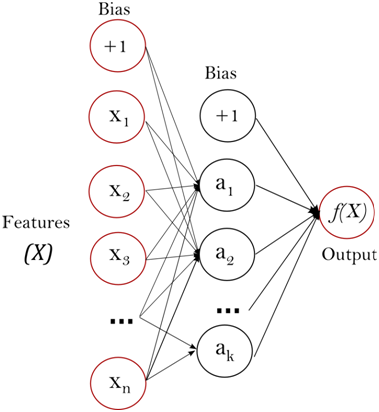
\includegraphics[width=0.5\linewidth]{perceptron.png}
\caption{Three-layer perceptron with scalar output (source https://scikit-learn.org)}
\label{fig1}
\end{center}
\end{figure}   

The left layer called the \textit{input} one consists of a set of neurons $x_i, \; i=\overline{1,n}$ representing the input signals (the values of variables). Each neuron in the hidden layer transforms the values from the previous layer with weighted linear summing 
\[
w_1 x_1 + w_2 x_2+...+w_n x_n+bias,
\]
where $w_i$ are the weights of the neurons and $bias$ is a special weight, which doesn't include a factor in the form of an input value. Next, the value obtained is transformed into an output one (predicted) value of the layer with a transmission function (the \textit{activation function}). The output layer receives the values from the last hidden layer and transforms these ones onto the output values. The network was trained by the error backpropagation method.

\subsubsection{Selection of the Model Parameters}

The choice of the solver, the activation function, the value of the regularization parameter, the number of neurons in the hidden layer, etc. are the variable adjustment parameters of the neural network.
For example, for small sets of the multidimensional data ``lbfgs'' solver was demonstrated to be better and faster. This solver is a modification of Broyden-Fletcher-Goldfarb-Shanno algorithm \cite{Nocedal2006} and belongs to the quasi-Newton methods. All numerical experiments were carried out using this algorithm.
The sigmoidal functions (logistic or hyperbolic tangent) were used as the neuron activation ones.
The number of neurons in each layer and the regularization parameter (alpha) were adjusted in the experiments and depended on particular problem.

In the experiments conducted, we selected the following network architecture:
\begin{verbatim}
model = MLPRegressor(activation='logistic',
	solver='lbfgs',
	alpha=0.001,
	hidden_layer_sizes=(20,),
	max_iter=5000,
	tol=10e-6,
	random_state=10)
\end{verbatim}


\subsection{The Use of Approximations in Solving the Optimization Problem}\label{GSA_Appr}

In the present study, we applied the following method of using the objective function approximation in the optimization problems: to construct the objective function approximation using the accumulated search information, to find the minimum of the approximation, and to repeat this process either until the computation resources is exhausted or until the convergence is achieved.

The method proposed will make sense either in the case when the amount of the search information accumulated is large enough (that allows constructing a relatively precise approximation of a multiextremal function) or in the case when the problem is similar to a local extremum search one.
The first case corresponds to the final stage of search and can be interpreted as a method of refining current solution. However, if the objective function is a time-consuming one, it is impossible to conduct large enough number of trials. Here we shall meet the computational resources exhausted.

The second case implies a construction of a good approximation based on relatively small number of trials and in fact includes an assumption on a weak muliextremality of the objective function that matches the problem considered within the framework of the present study well.
 
The global search algorithm using the objective function approximation can be formulated as follows.
Let us assume the resources available to allow performing $K_{max} = K_1 + K_2$ trials.

At the first stage, $k = K_1$ trials are performed using core global search algorithm from section \ref{GSA}.
In the course of performing the first stage, a set of the trial results $\Omega = \left\{(y^k, \varphi(y^k)), 0\leq k\leq K_1\right\}$ necessary to construct the objective function approximation is accumulated.

At the second stage, the algorithm works using the approximation. To compute the point $y^{k+1}$ of the next $(k+1)^{\rm th}$ trial, the following operations are performed.

%Описание работы алгоритма
Step 1. Using the set of the trial results $\Omega$ formed in the course of the algorithm execution, to construct an approximation of the objective function $\overline{\varphi}(y)$;

Step 2. Using core global search algorithm from section \ref{GSA}, to find the global minimum of the function $\overline{\varphi}(y)$ and to use this value as the next trial point i. e. $y^{k+1} = \arg \min_{y \in D} \overline{\varphi}(y)$.

Step 3. If either the condition $k>K_{max}$ or the one $\left\|y^k - y^{k+1}\right\| \leq \epsilon$ is satisfied, to stop the algorithm.
Else, to perform the trial at the point $y^{k+1}$, to store its result in the set $\Omega$, to increment the trial counter $k = k+1$, and to proceed to Step 1.

The algorithm proposed here ensures the convergence to the global solution in the case if $K_1$ trials executed at the first stage is enough to construct an approximation of the objective function reflecting the main features of its behavior adequately.

%пример работы алгоирмта на тестовой задаче?

%%%%%%%%%%%%%%%%%%%%%%%%%%%%%%%%%%%%%%%%%%

%\subsection{Loss function definition}

%%%%%%%%%%%%%%%%%%%%%%%%%%%%%%%%%%%%%%%%%%
\section{Results}

%Описание оборудования и программного обеспечения, которое было задействовано при проведении экспериментов.

%Результаты расчетов

%Иллюстрации

%Сравнение нескольких разных решений (это можно перенести и в следующую секцию)

The simulations were conducted using supercomputer of Lobachevsky University of Nizhni Novgorod (operated under Linux CentOS 7.2 operation system). Each cluster node included two  Intel Sandy Bridge E5-2660 2.2 GHz processors, 64 Gb RAM; the central processor unit had 8 cores. 
The global optimization methods considered in the present work were implemented in C++ using GCC 5.5.0 compiler and Open MPI v4.1.1. To construct the objective function approximations using a neural network, scikit-learn machine learning library from Python 3.9 was applied. 
For the numerical solving of the problem described in Section \ref{math_model}, open source CFD software OpenFOAM v2012 \cite{OpenFOAM} was used.


%В процессе оптимизации исследовались такие константы, как $\beta^*$, $a_1$, $\alpha_{k 1,2}$, $\alpha_{\omega 1,2}$, которые регулируют скорость диссипации турбулентной кинетической энергии, напряжения Рейнольдса, поток диффузии турбулентной кинетической энергии, поток диффузии диссипации турбулентной кинетической энергии, соответственно.
Such constants of the turbulence model as $\beta^*$, $a_1$, $\alpha_{k 1,2}$, $\alpha_{\omega 1,2}$ have been optimized. They regulate the turbulent kinetic energy dissipation rate, Reynolds stress, turbulent kinetic energy diffusion flux, diffusion flux of turbulent kinetic energy dissipation, respectively.

%Начальные значения коэффициентов были заданы следующими:
The initial values of the coefficients are
\begin{equation}
	\begin{aligned}
		\beta^* = 0.09;\ \ \ a_1 = 0.31;\ \ \ \alpha_{k 1} = 0.85;\ \ \ \alpha_{\omega 1} = 0.5; \ \ \ \alpha_{k 2} = 1.0;\ \ \ \alpha_{\omega 2} = 0.856.
	\end{aligned}
\end{equation}
One calculation of the objective function at given values of parameters took 15 minutes in average with the use of 8 MPI-processes per a node. 

The optimal values of parameters were adjusted for pairs, the values of the rest parameters were fixed. 
First, a pair of the most important parameters $\beta^*$ and $a_1$ was selected. 
To investigate the optimization problem arising, both possible approaches to solving the one were applied: without the use of the objective function approximation  and with the use of the approximation.

In the first experiment, the global search algorithm described in subsection \ref{GSA} was applied without the use of approximation. 
The parameters of the method were set $r = 3$ and $\epsilon = 10^{-3}$. 
In 24 hours, 100 iterations of the algorithm were performed; the required accuracy was not achieved. 

In the second experiment, the approach described in subsection \ref{GSA_Appr} was applied to solve the same problem.
First, $K_1 = 30$ iterations of global search algorithm were performed. 
Afterwards, the algorithm employing the approximation with the neural network was started. 
Total $K_1 + K_2 = 65$ iterations of the algorithm were performed, after that the algorithm stopped on accuracy. 
As a result, the best value  of the objective function 0.375174 was found. 
Total solution search time was reduced down to 16 hours that provided obtaining more accurate solution of the problem in acceptable time.

The trial points and the approximating function plotted according to these points using the neural network are presented in Figure~\ref{NN_100_point} (the parameters $\beta^*$ and $a_1$ were varied). One can see clearly several local minima to be present.

\begin{figure}[H]
\begin{center}
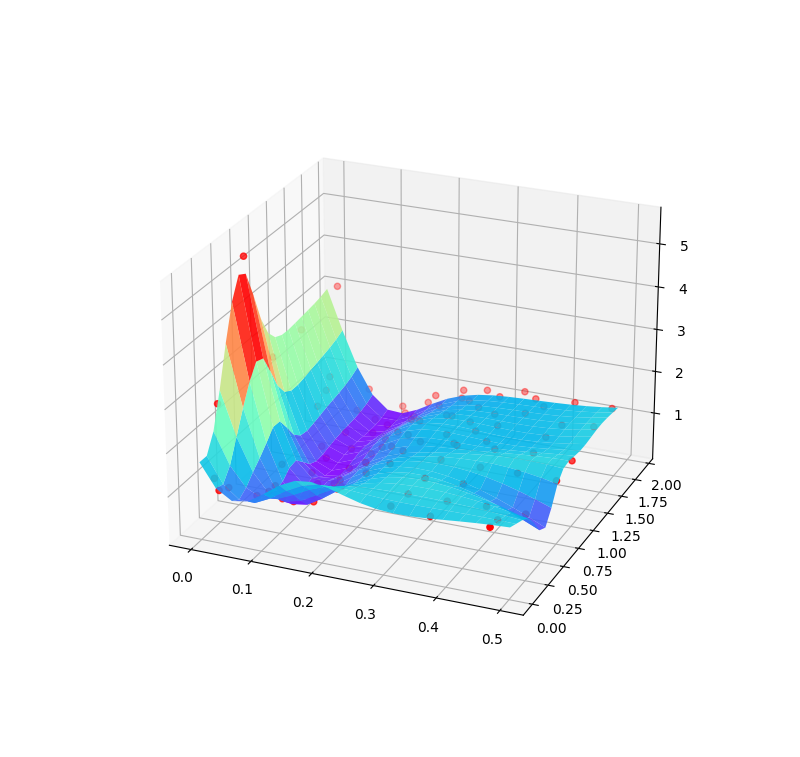
\includegraphics[width=0.8\linewidth]{NN_100_point_.png}
\caption{Objective function values (red points) and approximation plot constructed using the neural network (parameters $\beta^*$ and $a_1$ were varied)}
\label{NN_100_point}
\end{center}
\end{figure}

The best values of parameters $\beta^*$ and $a_1$ found were fixed, and then optimization in parameters $\alpha_{k1}, \alpha_{\omega1}$, and $\alpha_{k2}, \alpha_{\omega2}$ was performed. 
The optimization in these parameters didn't result in a considerable improvement of the objective function: the value of 0.364464 was obtained.


%На рисунках ~\ref{NN_100_point1} и ~\ref{NN_100_point2} приведены изображение функций, полученные с помощью аппроксимации задачи нейросетью, обученной на 100 точках испытания, варьировались соответсвенно пары параметров $\alpha_{k1} $,  $\alpha_{\omega1} $ и $\alpha_{k2} $, $\alpha_{\omega2} $.
%
%\begin{figure}[H]
%\begin{center}
%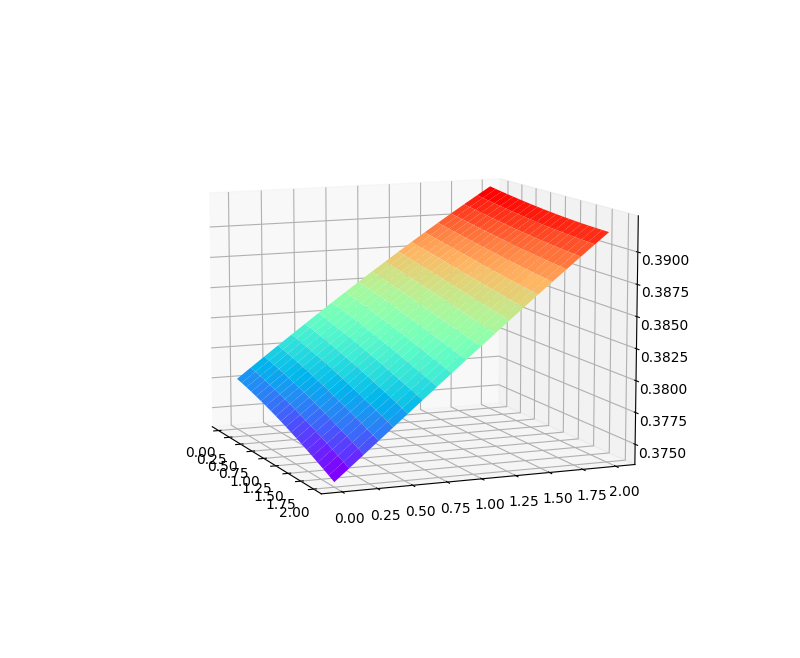
\includegraphics[width=1.0\linewidth]{ NN_100_point_1.png}
%\caption{Изображение функции, полученной с помощью аппроксимации задачи нейросетью, обученной на 100 точках испытания, варьировались параметры $\alpha_{k1} $ и $\alpha_{\omega1} $}
%\label{NN_100_point1}
%\end{center}
%\end{figure}
%
%\begin{figure}[H]
%\begin{center}
%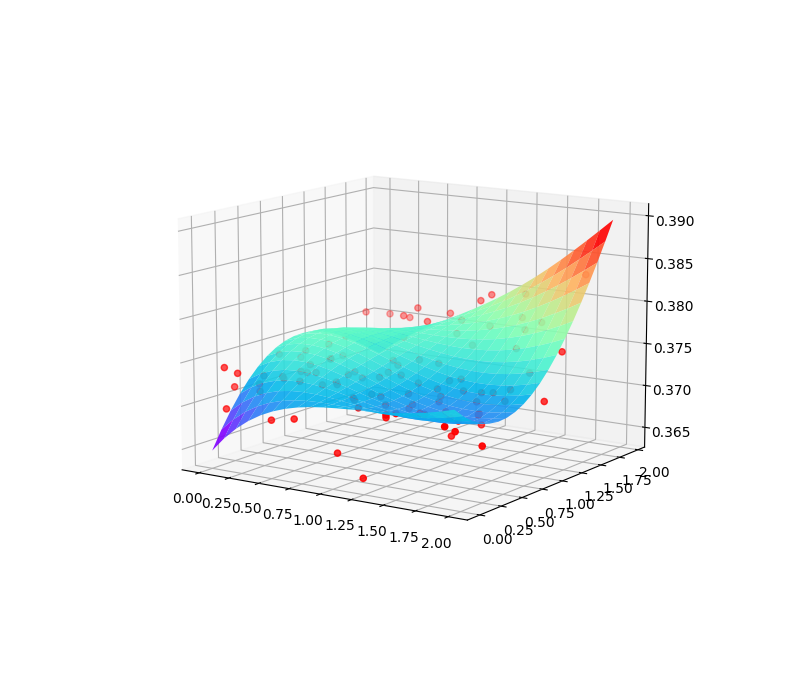
\includegraphics[width=1.0\linewidth]{ NN_100_point_tanh_alpha2_0.0001_.png}
%\caption{Изображение функции, полученной с помощью аппроксимации задачи нейросетью, обученной на 100 точках испытания, варьировались параметры $\alpha_{k2} $ и $\alpha_{\omega2} $}
%\label{NN_100_point2}
%\end{center}
%\end{figure}

%После калибровки значения коэффициентов стали следующими:
%The optimized values of the coefficients:
As a final result, the following values of the coefficients of the model were obtained:
\begin{equation}
	\begin{aligned}
		\beta^* = 0.117432;\ \ \ a_1 = 1.84082;\ \ \ \alpha_{k 1} = 1.999023;\\
		\alpha_{\omega 1} = 0.061523; \ \ \ \alpha_{k 2} = 1.241211;\ \ \ \alpha_{\omega 2} = 0.002930.
	\end{aligned}
\end{equation}

%Были получены следующие профили скорости на выходной плоскости для различных углов наклона лотка, как показано на рис.~\ref{NIIMexUProfilesKWSSTGlob}
Figure~\ref{NIIMexUProfilesKWSSTGlob} shows the resulting velocity profiles on the exit plane for various slope angles.

\end{paracol}
\nointerlineskip
\begin{figure}[H]	
\widefigure
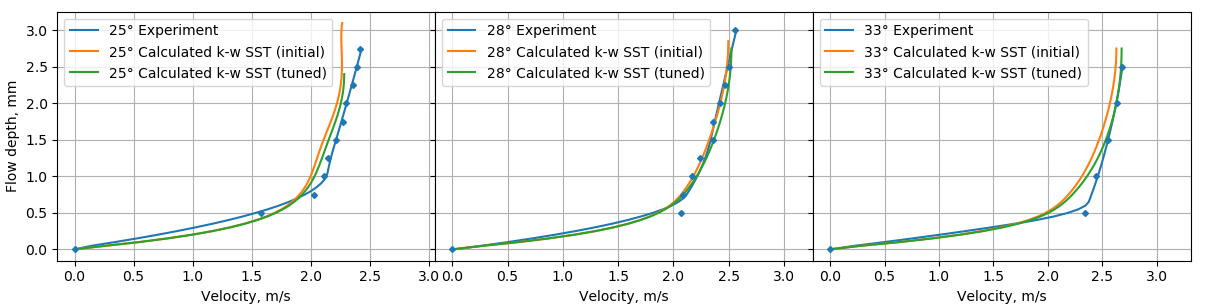
\includegraphics[width=18 cm]{UProfilesKWSSTGlob1.png}
\caption{Comparison of the experimental velocity profile with the calculated one using the standard values of the $k-\omega\ SST$ turbulence model coefficients and the calculated velocity profile with calibrated values of the coefficients for different slope inclination angles (to the horizon).\label{NIIMexUProfilesKWSSTGlob}}
\end{figure}  
\begin{paracol}{2}
\linenumbers
\switchcolumn

%Калибровка привела к следующей минимизации функции потерь~\eqref{LossFunction}, показанной в таб.~\ref{tabLossFunctionMinimize}
During the calibration, the following minimization of the loss function~\eqref{LossFunction} was achieved, as shown in Table~\ref{tabLossFunctionMinimize}.

%\begin{table}[H]
%	\caption{Минимизация функции потерь}
%	\label{tabLossFunctionMinimize}
%	\begin{center}
%		\begin{tabular}{ | c | m{0.3\textwidth} | m{0.3\textwidth} | } 
%			\hline
%			Угол наклона лотка& Начальное значение функции потерь & Минимизированное значение функции потерь\\
%			\hline
%			25$^\circ$ & 0.165 & 0.155\\
%			\hline
%			28$^\circ$ & 0.085 & 0.128\\
%			\hline
%			33$^\circ$ & 0.150 & 0.089\\
%			\hline
%		\end{tabular}
%	\end{center}
%\end{table}
\begin{specialtable}[H] 
    \caption{Loss function minimization\label{tabLossFunctionMinimize}}
    \begin{tabular}{  c  c  c  }
    \toprule
    \textbf{Slope angle} & \textbf{Initial value of loss function} & \textbf{Minimized value of loss function}\\
    \midrule
    25$^\circ$ & 0.165 & 0.155\\
    28$^\circ$ & 0.085 & 0.128\\
    33$^\circ$ & 0.150 & 0.089\\
    \bottomrule
    \end{tabular}
\end{specialtable}

%На рисунке \ref{NIIMexUProfilesKWSSTGlob} и в таблице \ref{tabLossFunctionMinimizeKE} можем видеть, что для двух углов наклона из трёх мы видим уменьшение расхождения расчётного профиля скорости с экспериментальным. Оптимизация по трём экспериментам одновременно (их функции потерь суммировались) использовалась с целью избежать переобучения модели, так как при использовании одного эксперимента, может быть достигнуто почти идеальное совпадение расчётного профиля скорости с экспериментальным, которое не воспроизводится на других экспериментах. Так же стоит отметить, что расхождение профиля скорости в области вблизи дна обусловлено погрешностью измерений в эксперименте, так как замер скорости с помощью трубки Пито, используемой в данном эксперименте, в непосредственной близости ото дна затруднён.
Figure~\ref{NIIMexUProfilesKWSSTGlob} and Table~\ref{tabLossFunctionMinimize} show that a decrease in the discrepancy between the calculated velocity profile and the experimental one for two out of three experiments. Optimization for three experiments altogether (their loss functions were summarized) was used in order to avoid the model overfitting. When using one experiment, an almost perfect coincidence of the calculated velocity profile with the experimental one is achieved, which is not reproduced in other experiments. It should also be noted that the divergence of the velocity profile in the region near the chute bottom is due to the measurement error in the experiment, since the measurement of the velocity using the Pitot tube used in this experiment in the immediate vicinity of the bottom is difficult.


%%%%%%%%%%%%%%%%%%%%%%%%%%%%%%%%%%%%%%%%%%
\section{Conclusions}

In this work, a two-phase flow in a chute was simulated using the interFoam solver, the URANS mathematical model, and the $k-\omega\ SST$ turbulence model. In the optimization process, six constants were investigated in pairs, which make the greatest contribution to the value of turbulent viscosity.

The comparison of the results of calculating the velocity profiles with the experimental data obtained at Research Institute of Mechanics, Moscow State University in different sections subject to the angle of inclination of the chute was conducted. The search for the optimal coefficients of the turbulence model was performed by minimizing the objective function of the divergence of the velocity profile in the chute. % - RMSE.

The search for the global minimum of the objective function was performed using the global search algorithm implemented in Globalizer software \cite{globalizerSystem}. In addition, a fully connected neural network with one hidden layer was used to approximate the values of the objective function by the values of the constants of the turbulent model. The MLPRegressor class from the scikit-learn library was used to build the objective function approximation. 

In the present work, an interdisciplinary approach was utilized, which helped us to find the optimal values of six turbulence model parameters using OpenFOAM open platform and Globalizer. The minimum value for the objective function was obtained in the case of the tray angle of 33 degrees. One calculation of the objective function for given parameters took 15 minutes in average using 8 MPI processes on a node of Lobachevsky University supercomputer. Total computation time was 24 hours.  




%%%%%%%%%%%%%%%%%%%%%%%%%%%%%%%%%%%%%%%%%%
%\section{Patents}
%
%This section is not mandatory, but may be added if there are patents resulting from the work reported in this manuscript.

%%%%%%%%%%%%%%%%%%%%%%%%%%%%%%%%%%%%%%%%%%
\vspace{6pt} 

%%%%%%%%%%%%%%%%%%%%%%%%%%%%%%%%%%%%%%%%%%
%% optional
%\supplementary{The following are available online at \linksupplementary{s1}, Figure S1: title, Table S1: title, Video S1: title.}

% Only for the journal Methods and Protocols:
% If you wish to submit a video article, please do so with any other supplementary material.
% \supplementary{The following are available at \linksupplementary{s1}, Figure S1: title, Table S1: title, Video S1: title. A supporting video article is available at doi: link.} 

%%%%%%%%%%%%%%%%%%%%%%%%%%%%%%%%%%%%%%%%%%
\authorcontributions{Conceptualization, K.B. and D.R.; methodology, Rom.D. and K.B.; software, I.L., D.R., M.U. and  Rom. D.; validation,  Rom.D. and I.L.; formal analysis, S.S., M.U.; investigation, S.S.; resources, I.L.; data curation, Rom.D. and M.U.; writing---original draft preparation, K.B., S.S. and Rom.D.; writing---review and editing, R.D.; visualization, I.L.; supervision, S.S.; project administration, K.B.; funding acquisition, S.S. All authors have read and agreed to the published version of the manuscript.}

\funding{This research was supported by the Ministry of Science and Higher Education of the Russian Federation, agreement No 075-15-2020-808.}

\institutionalreview{Not applicable.}

\informedconsent{Not applicable.}

%\dataavailability{In this section, please provide details regarding where data supporting reported results can be found, including links to publicly archived datasets analyzed or generated during the study. Please refer to suggested Data Availability Statements in section ``MDPI Research Data Policies'' at \url{https://www.mdpi.com/ethics}. You might choose to exclude this statement if the study did not report any data.} 

\acknowledgments{The authors consider it their duty to acknowledge the contribution of prof. Victor Gergel (14.01.1955 -- 29.06.2021), who initiated this interdisciplinary study.}

\conflictsofinterest{The authors declare no conflict of interest.} 

%% Optional
%\sampleavailability{Samples of the compounds ... are available from the authors.}

%%%%%%%%%%%%%%%%%%%%%%%%%%%%%%%%%%%%%%%%%%
%% Only for journal Encyclopedia
%\entrylink{The Link to this entry published on the encyclopedia platform.}

%%%%%%%%%%%%%%%%%%%%%%%%%%%%%%%%%%%%%%%%%%
%% Optional
%\abbreviations{The following abbreviations are used in this manuscript:\\

%\noindent 
%\begin{tabular}{@{}ll}
%MDPI & Multidisciplinary Digital Publishing Institute\\
%DOAJ & Directory of open access journals\\
%TLA & Three letter acronym\\
%LD & Linear dichroism
%\end{tabular}}
%
%%%%%%%%%%%%%%%%%%%%%%%%%%%%%%%%%%%%%%%%%%%
%%% Optional
%\appendixtitles{no} % Leave argument "no" if all appendix headings stay EMPTY (then no dot is printed after "Appendix A"). If the appendix sections contain a heading then change the argument to "yes".
%\appendixstart
%\appendix
%\section{}
%\subsection{}
%The appendix is an optional section that can contain details and data supplemental to the main text---for example, explanations of experimental details that would disrupt the flow of the main text but nonetheless remain crucial to understanding and reproducing the research shown; figures of replicates for experiments of which representative data are shown in the main text can be added here if brief, or as Supplementary Data. Mathematical proofs of results not central to the paper can be added as an appendix.
%
%\begin{specialtable}[H] 
%%\tablesize{\scriptsize}
%\caption{This is a table caption. Tables should be placed in the main text near to the first time they are~cited.\label{tab1}}
%%\tablesize{} % You can specify the fontsize here, e.g., \tablesize{\footnotesize}. If commented out \small will be used.
%\begin{tabular}{ccc}
%\toprule
%\textbf{Title 1}	& \textbf{Title 2}	& \textbf{Title 3}\\
%\midrule
%Entry 1		& Data			& Data\\
%Entry 2		& Data			& Data\\
%\bottomrule
%\end{tabular}
%\end{specialtable}
%
%\section{}
%All appendix sections must be cited in the main text. In the appendices, Figures, Tables, etc. should be labeled, starting with ``A''---e.g., Figure A1, Figure A2, etc. 

%%%%%%%%%%%%%%%%%%%%%%%%%%%%%%%%%%%%%%%%%%
\end{paracol}
\reftitle{References}

% Please provide either the correct journal abbreviation (e.g. according to the “List of Title Word Abbreviations” http://www.issn.org/services/online-services/access-to-the-ltwa/) or the full name of the journal.
% Citations and References in Supplementary files are permitted provided that they also appear in the reference list here. 

%=====================================
% References, variant A: external bibliography
%=====================================
\externalbibliography{yes}
\bibliography{bibliography}

%=====================================
% References, variant B: internal bibliography
%=====================================
%\begin{thebibliography}{999}
%% Reference 1
%\bibitem[Author1(year)]{ref-journal}
%Author~1, T. The title of the cited article. {\em Journal Abbreviation} {\bf 2008}, {\em 10}, 142--149.
%% Reference 2
%\bibitem[Author2(year)]{ref-book1}
%Author~2, L. The title of the cited contribution. In {\em The Book Title}; Editor1, F., Editor2, A., Eds.; Publishing House: City, Country, 2007; pp. 32--58.
%% Reference 3
%\bibitem[Author3(year)]{ref-book2}
%Author 1, A.; Author 2, B. \textit{Book Title}, 3rd ed.; Publisher: Publisher Location, Country, 2008; pp. 154--196.
%% Reference 4
%\bibitem[Author4(year)]{ref-unpublish}
%Author 1, A.B.; Author 2, C. Title of Unpublished Work. \textit{Abbreviated Journal Name} stage of publication (under review; accepted; in~press).
%% Reference 5
%\bibitem[Author5(year)]{ref-communication}
%Author 1, A.B. (University, City, State, Country); Author 2, C. (Institute, City, State, Country). Personal communication, 2012.
%% Reference 6
%\bibitem[Author6(year)]{ref-proceeding}
%Author 1, A.B.; Author 2, C.D.; Author 3, E.F. Title of Presentation. In Title of the Collected Work (if available), Proceedings of the Name of the Conference, Location of Conference, Country, Date of Conference; Editor 1, Editor 2, Eds. (if available); Publisher: City, Country, Year (if available); Abstract Number (optional), Pagination (optional).
%% Reference 7
%\bibitem[Author7(year)]{ref-thesis}
%Author 1, A.B. Title of Thesis. Level of Thesis, Degree-Granting University, Location of University, Date of Completion.
%% Reference 8
%\bibitem[Author8(year)]{ref-url}
%Title of Site. Available online: URL (accessed on Day Month Year).
%\end{thebibliography}

% If authors have biography, please use the format below
%\section*{Short Biography of Authors}
%\bio
%{\raisebox{-0.35cm}{\includegraphics[width=3.5cm,height=5.3cm,clip,keepaspectratio]{Definitions/author1.pdf}}}
%{\textbf{Firstname Lastname} Biography of first author}
%
%\bio
%{\raisebox{-0.35cm}{\includegraphics[width=3.5cm,height=5.3cm,clip,keepaspectratio]{Definitions/author2.jpg}}}
%{\textbf{Firstname Lastname} Biography of second author}

% The following MDPI journals use author-date citation: Arts, Econometrics, Economies, Genealogy, Humanities, IJFS, JRFM, Laws, Religions, Risks, Social Sciences. For those journals, please follow the formatting guidelines on http://www.mdpi.com/authors/references
% To cite two works by the same author: \citeauthor{ref-journal-1a} (\citeyear{ref-journal-1a}, \citeyear{ref-journal-1b}). This produces: Whittaker (1967, 1975)
% To cite two works by the same author with specific pages: \citeauthor{ref-journal-3a} (\citeyear{ref-journal-3a}, p. 328; \citeyear{ref-journal-3b}, p.475). This produces: Wong (1999, p. 328; 2000, p. 475)

%%%%%%%%%%%%%%%%%%%%%%%%%%%%%%%%%%%%%%%%%%
%% for journal Sci
%\reviewreports{\\
%Reviewer 1 comments and authors’ response\\
%Reviewer 2 comments and authors’ response\\
%Reviewer 3 comments and authors’ response
%}
%%%%%%%%%%%%%%%%%%%%%%%%%%%%%%%%%%%%%%%%%%
\end{document}

